% How to use R
% Author: Sam Pollard (sam.d.pollard@gmail.com)
% Last Modified: April 14, 2015

\documentclass[12pt]{article}
\usepackage[margin=1in, headheight=15pt]{geometry}
\usepackage{amsmath, amssymb, amsthm}
\frenchspacing % Single spacing after all periods.

% Remove the headrule and make enough space for the header
\usepackage{fancyhdr}
\renewcommand{\headrulewidth}{0pt}
\setlength{\headheight}{15pt} % If two lines in the header, make 30pt

\usepackage{graphicx, hyperref, fancyvrb}

\pagestyle{fancy}
\lhead{Learn you some R}
% If something is more than 1 page, add the page number. May require two compilations.
\usepackage{totcount}
\regtotcounter{page}
\cfoot{\ifnum\totvalue{page} > 1 \thepage \else\fi}

\theoremstyle{remark}
\newtheorem{exercise}{Exercise}

\begin{document}
\part{Learn You Some R, Practically}
\begin{center}
	\begin{Large}
	Sam Pollard
	\end{Large}
	\\
	\today
\end{center}
\section{Introduction}

This guide is meant for people with little or no programming experience. That being said, this guide moves quickly and is aimed towards people with technical training in some scientific field. There are many guides for programming which are aimed at computer scientists and use lots of jargon computer scientists have heard for years. This can be difficult to understand. On the other hand, many guides use such simple examples that you can't really do anything interesting with what you learn. This guide attempts to provide meaningful examples and explain the fundamental programming concepts which cannot be easily Googled. This guide comes with a supplementary R file which contains all of the example code used in this guide. If you have any feedback please mail me at \url{sam.d.pollard@gmail.com}

A word on notation: things written in \verb|this font| represent things which are typed exactly into R or the output of running commands. Things in \emph{this font} are either vocabulary used by R, mathematical notation, or emphasis added by me. It should be clear from the context.

R is what is called an \emph{open} project. That means that anyone can contribute to R. This results in a large number of what are called \emph{packages}, which consist of a bunch of R files which ``work together'' to provide a service. This also results in R being really really huge in terms of the number of features it provides.

To use R, you must first download and install it. I found the easiest way to do this is to go to \url{http://cran.cs.wwu.edu/}, which is hosted by Western Washington University. You then install it like any normal program.

There are two basic ways to work with R. One is in \emph{interactive} mode, the other is \emph{batch processing}. Batch processing is when R executes commands it reads from a text file. This text file is called \emph{source code} and by convention these files end with the \verb|.R| extension. This can be done in Windows by clicking \emph{File} then \emph{Source R Code\dots}. Alternatively, you can edit an R source file by clicking \emph{File} then \emph{Open Script}. Interactive mode is useful for temporary or scratch work, while batch processing is useful for reproducibility.

For example, you can run the file \verb|sample_code.R| provided via batch processing. This will run every command presented in this guide and save a few files in the same folder (a.k.a. directory) as the one where the source code is stored. This is far from being pedagogical because everything will finish in less than a second, but this behavior is critical for automating tasks.

When you start R the default behavior is to run in interactive mode. Below are a few sample commands in interactive mode. When R first starts in this manner it will display some text about what R is and how to exit. This has been omitted. As this guide progresses I recommend you execute each of the commands from the attached file \verb|learnR.R|. Don't worry if much of this doesn't make sense; each component will be explained.

\begin{Verbatim}[frame=single, fontsize=\small]
> data(trees) # Load a sample dataset
> nrow(trees) # Count the sample size
[1] 31
> colnames(trees)
[1] "Girth"  "Height" "Volume"
> max(trees["Volume"]) # Find the largest in the column
[1] 77
> max(trees[3]) # The same as above because we access the third column
[1] 77
> apply(trees, 2, mean)
   Girth   Height   Volume 
13.24839 76.00000 30.17097 
\end{Verbatim}

The symbol \verb|>| is called a \emph{prompt}, which is the interpreter's (we'll define what that is later) way of saying, ``I'm ready to process another command.'' Anything following a \# is a comment. This is to make the commands more human-readable, but are ignored by R entirely.

The \verb|[1]| symbol is a way of saying, ``here is the first element of the output which you're not storing anywhere.''\footnote{Technically, it refers to the first element of a one-element vector. These will be explained later.} As we will see, it is common to store the output (or \emph{return value}) of a function call in a variable. This is explained in the next section, but in this example the return value of the function calls are just printed\footnote{It is common when programming to use ``print'' for describing something displayed on the screen instead of just something physically printed.} for the user to view.

It is important to keep in mind while programming R that almost everything is a function call. Functions in R are much more general and abstract than what the average person (read: non-mathematician) has learned about functions. In math we write $f(x, y) = x^2 + y^2$ to describe a function $f$ which takes in two numbers and returns a third number. Functions in R don't need to just take as input numbers. For example, \verb|trees| is not a number but rather a table of numbers. Functions are so important in R that after reading this guide the word ``function'' might sound weird. In fact, functions are so important that they deserve their own section (Section \ref{functions}). But first, we need to understand our first example.

Typing a function in R is the same as in math: the function name followed by the arguments (or inputs) in parentheses. For example, we have something like \verb|nrow(trees)| which takes as input the variable \verb|trees| and returns the number of rows that variable contains.

The last command is a bit complicated but fits with intuition. The \verb|apply| function takes as an argument some \emph{data frame} (in this case \verb|trees|), a 1 or 2 (1 for rows, 2 for columns), and a function (\verb|mean| here), and applies that function to each row or column in the data set. It is generally considered good practice to use built-in functions such as \verb|apply| because they make code easier to understand and maintain.

\section{Basic Syntax and Examples}

R is what is called an \emph{interpreted} language. This means that there is an aptly-named \emph{interpreter} which keeps track of all the variables you have and how to execute the commands you type. The benefit to being interpreted is you have the flexibility of running one line at a time and thus can easily run in interactive mode.

One potential drawback of an interpreted language is it can be difficult to find the errors in your code, because they may not be detected until the source code is run. This can be mitigated by testing small chunks of your code as you write it.

In the first example, the object \verb|trees| is what is called a \emph{data frame}. In R, this is denoted \verb|data.frame|. This can be thought of as your typical spreadsheet format: A list of a bunch of columns. The one restriction is that each column must have equal length. Here is a quick example:

\begin{Verbatim}[frame=single, fontsize=\small,  numbers=left]
> name <- c("H","He","Li")       # c can be thought of as "combine"
> mass <- c(1.0079,4.0026,6.941) # i.e. make a vector from the arguments
> atomic_number <- seq(1,length(name))
> mydf <- data.frame(atomic_number, name, mass)
> mydf                           # Print out the data.frame
  atomic_number name   mass
1             1    H 1.0079
2             2   He 4.0026
3             3   Li 6.9410
\end{Verbatim}

A few remarks are in order. The most fundamental is the effect of \verb|<-|. This performs an \emph{assignment} of the right-hand value to the left-hand value. The assignment on line 1 creates a variable called \verb|name| and puts a value inside of it. The \verb|<-| symbol is read as ``gets.'' This is the official way to perform assignment, but you will often see code such as \verb|name=c("H","He","Li")| instead, which is also assignment (this is common syntax in other programming languages). I recommend using \verb|<-| because \verb|=| is used in another context in R so this clarifies the distinction. The fourth line calls the \verb|data.frame| function which takes as input some number of vectors and returns a data frame. This return value is stored in the variable \verb|mydf|.  The name, mass, and atomic\_number form the \emph{header} (also known as column names) of the data frame.

Unlike most other programming languages, the period can be used in variable names. It is typically used to denote a more specific way to go about things. For example, the function \verb|read| is used in a lot of contexts: It can be used to ask the user for input, it can read files, and many other things. A very useful ``version'' of \verb|read| is \verb|read.csv|, which takes in a csv file and turns it into a data frame.

Consider the following example, which reads a csv and allows us to use all of R's features to analyze the data contained within:

\begin{verbatim}
> mydf <- read.csv("report.csv", header = TRUE, sep = ",")
\end{verbatim}

The \verb|read.csv| function takes in at least 1 argument: the file name. Three are given above to give more specification about how we want to read the csv file. To prevent R from interpreting \verb|report.csv| as a variable, the value is closed in quotes\footnote{A bunch of letters enclosed within quotes is called a \emph{string}. Here are some examples of strings: \texttt{"Hello"}, \texttt{"121a.a;lk!"}.}.
The \verb|header = TRUE| indicates that the first line of this csv file contains the names of each column. If this is set to \verb|FALSE|, R sets the column names to \verb|V1|, \verb|V2|, and so on. The last argument is the \emph{separator}. This may be whatever you want. Cryptically, a csv (comma separated value) file may not be separated by commas. Oftentimes, it is tab-separated. To accommodate this, one can say \verb|sep = "\t"|. The backslash here \emph{escapes} the succeeding character \verb|t| and instead interprets this as a tab.

\section{Some Subtleties}
\subsection{Vectors}
The previous example used the \verb|c| function. This is used is to put data in the correct format. This is an important part of R and programming in general. The distinction here is between a \emph{vector} and a \emph{scalar}. This fits with mathematical intuition but not so much with the real world. Ask a mathematician what a vector is and she will respond, ``It is something that behaves like a vector.'' While this is sort of a joke, there really isn't any better definition. In R, vectors are all over the place. Here are some examples and a non-example (can you spot which?)
\begin{Verbatim}[frame=single, fontsize=\small]
n <- nrow(trees)           # The number of trees
tag <- seq(1,n)            # A sequence from 1 to n, inclusive
lifespan <- 70*runif(n)    # Random values between 0 and 70, inclusive
volume <- trees["Volume"]  # The volume of each tree
\end{Verbatim}

The last example is \emph{not} a vector. It is a data frame. This means things that require vectors won't work on the data frame. For example,
\begin{verbatim}
> mean(volume)
[1] NA
\end{verbatim}

However, if we make a small modification:
\begin{verbatim}
> volumevec <- trees[["Volume"]]
\end{verbatim}
This \emph{is} a vector.

If you're stuck, the \verb|class| function may describe what sort of data you're dealing with. Another useful method is \verb|ls()| which lists all the variables in your current workspace.

But what about the first example? Is it a vector? In some sense, yes. A vector can have one element. It is easiest to think of a scalar as the special vector which has one element. In general, most things you can do with scalars you can do with vectors. For example,
\begin{verbatim}
> lifespan <- lifespan + 15
\end{verbatim}
would increase the \verb|lifespan| variable by 15 (add 15 to each element in lifespan). Notice that this statement contains lifespan on the right-hand side and the left-hand side. In English we would say, ``take each element in lifespan and add 15 to it, storing the result in the variable lifespan.''

\subsection{Building Up}
A common task when working with spreadsheets is combining data from multiple sources into a single structure. Here, we will look at the \verb|cbind|, and \verb|paste| functions. We will keep using our previous examples and create a data frame which represents all of the vectors we have created. We begin this somewhat contrived example by creating ``names'' for each of the trees.

\begin{verbatim}
> treenames <- paste("T", tag, sep = "")
\end{verbatim}

This creates a sequence of strings. Notice that R is smart enough to determine that while you only specified a single string ``T'' (instead of a vector of strings of the same length as \verb|tag|), it concatenates ``T'' with each element of \verb|tag|. For example, tree 15 would be named \verb|T15|.

Now, to create a new data frame from the existing data we created, try
\begin{verbatim}
> mydf <- cbind(treenames, trees, lifespan)
\end{verbatim}
This is close to what we want. The function \verb|cbind| takes as input data frames or vectors, and combines them by \verb|c|olumn into a new data frame. There is an analogous function called \verb|rbind| which combines the data by row. Here is what the first few entries look like:

\begin{Verbatim}[frame=single, fontsize=\small]
> head(mydf)
  treenames Girth Height Volume lifespan
1        T1   8.3     70   10.3 15.18891
2        T2   8.6     65   10.3 15.85794
3        T3   8.8     63   10.2 15.41223
4        T4  10.5     72   16.4 15.30183
5        T5  10.7     81   18.8 15.86208
6        T6  10.8     83   19.7 15.87640
\end{Verbatim}
By the way, \verb|head| is a nice way to just see the beginning of a data frame (it is common to deal with thousands of rows of data). But this doesn't look quite right: the row names are just 1, 2, 3, \dots but we want them to represent our cleverly named tree names. R allows us to change row names and column names using the aptly named functions \verb|rownames| and \verb|colnames|. So,
\begin{verbatim}
> rownames(mydf) <- treenames
\end{verbatim}
We can also retrieve the row or column names by putting this function call on the right-hand side of an assignment like so: \verb|names <- rownames(mydf)|. To anyone with programming experience, this is a bit strange. The function can be used both as an \emph{l}-value, a.k.a. the left-hand side of an assignment statement a.k.a. the location of the variable getting changed, and an \emph{r}-value, a.k.a. the right-hand side of an assignment statement a.k.a. the return value of a function call. This is where the \verb|<-| notation keeps us sane: it directs us where the data we computed is being stored.

However, this data frame still looks a bit off:
\begin{Verbatim}[frame=single, fontsize=\small]
> head(mydf)
   treenames Girth Height Volume lifespan
T1        T1   8.3     70   10.3 15.18891
T2        T2   8.6     65   10.3 15.85794
T3        T3   8.8     63   10.2 15.41223
T4        T4  10.5     72   16.4 15.30183
T5        T5  10.7     81   18.8 15.86208
T6        T6  10.8     83   19.7 15.87640
\end{Verbatim}
Let's delete that first row:
\begin{verbatim}
> mydf <- mydf[,-1]
\end{verbatim}

That is some cryptic R code. There are other ways to accomplish the same task, but this one easily generalizes. In general, we access things by \verb|[row, column]|. So by default, we are accessing \emph{every} row. That is, there is nothing preceding the comma. Now, we are accessing every column but the first one (think of \verb|-| as removing the first column). Alternatively, we could \emph{include} every other column. So
\begin{verbatim}
> mydf <- mydf[,c(2,3,4,5)]
\end{verbatim}
would accomplish the same task. If we only cared about a few rows of \verb|mydf| we could write
\begin{verbatim}
> sample <- mydf[seq(4,9),]
\end{verbatim}
This takes the 4th through 9th rows of \verb|mydf|, inclusive.

\subsection{Default Parameters}
Returning to the first example of creating the tree names, we had to specify that \verb|sep = ""|, or the \emph{empty string}. If this was left out, i.e. \verb|paste("T",tag)|, then by default the strings are concatenated using a space as separator. We would get \verb|T 15| instead of \verb|T15|. Why is this? The motivation behind this is that most of the time a user will want the values separated by spaces. Without anything, there is the \emph{default parameter} for \verb|sep|, which is a space. Parameter specification takes the general form \verb|tag = value|, where \verb|tag| is specific to the function being called and \verb|value| can be anything you want, though not every value is correct in every circumstance. This appears all over the place in R programs, and here we don't have the choice to use \verb|<-|.

\section{Regression and Plotting}

This section will first gather some data and curves to be plot using R's regression features. These will be plotted but the output will be the default, plain format. Next, more advanced plotting features will be exploited to improve the quality of the figures and allow saving of the figures in multiple file formats.

\subsection{Regression}
Below is an extended example which plots a bunch of (simulated) noisy data and fits a curve to it. Which realistically is the solution to about half of all scientific problems.

\begin{Verbatim}[frame=single, fontsize=\small, numbers=left]
lb <- 0     # The lower and upper bounds will be used repeatedly
ub <- 10
time <- seq(from = lb, to = ub, length.out = 100)
noisy_data <- rnorm(100, mean = 0, sd = 5) + 10 # Equivalently: rnorm(100,10,5)
noisy_data <- abs(noisy_data) + time^2
# Make a scatterplot of the data
plot(time, noisy_data)
\end{Verbatim}

The first two lines create some made up data. Specifically, the ``noise'' is simulated with a normal distribution with mean 0 and standard deviation 5. Taking the absolute value of the data (\verb|abs| on line 5) will be nice a bit later when we want to interpret and plot the data. Since the 10 is added in line 4, this puts the mean at 15. Line 5 adds this noisy data to the square of a sequence of 100 elements going from 0 to 10. For example, \verb|time[1]^2 = 0|, \verb|time[2]^2 = 0.0102|, \dots, \verb|time[99]^2 = 97.99|, and \verb|time[100]^2 = 100| . We have seen \verb|seq| before and this is a more general use of the function. Squaring the points created from \verb|seq| gives points from the quadratic $f(x) = x^2$. Putting this all together means the noisy data \emph{should} be best fit by the curve $x^2 + 10$. Hopefully, a least-squares approximation will yield a curve close to that.

However, since we know from what distribution the data is sampled, we are dealing in some sense with a ``solved'' problem. Suppose for a while that we don't know the underlying distribution of the data. A valid technique would be to guess the data fits some linear model.

\begin{Verbatim}[frame=single, fontsize=\small, numbers=left]
linearmodel <- lm(noisy_data ~ time)
# Get the coefficients to overlay the best-fit line over the scatterplot
intercept <- coef(linearmodel)[1]
slope <- coef(linearmodel)[2]
curve(slope * x + intercept, add = TRUE)
\end{Verbatim}

Line 1 attempts to fit a linear model to the data. The \verb|~| character (tilde) indicates a \emph{formula} is used. With a linear model, the parameters are implied. That is, \verb|lm| reads in the simple expression \verb|noisy_data ~ time| and from it knows both the the data on which a regression should be performed and the approximate form of the equation. \verb|lm| is attempting to find the best $m$ and $b$ which satisfy the equation $f(t) = mt + b$ where $f(t)$ is the noisy data and $t$ is time. Here, $m$ and $b$ are the \emph{coefficients}. Let's see how a linear model fits:

\begin{Verbatim}[frame=single, fontsize=\small]
> summary(linearmodel)

Call:
lm(formula = noisy_data ~ time)

Residuals:
    Min      1Q  Median      3Q     Max 
-16.658  -6.204  -1.393   6.674  21.740 

Coefficients:
            Estimate Std. Error t value Pr(>|t|)    
(Intercept)  -6.3943     1.8774  -3.406 0.000957 ***
time         10.0070     0.3244  30.852  < 2e-16 ***
---
Signif. codes:  0 '***' 0.001 '**' 0.01 '*' 0.05 '.' 0.1 ' ' 1

Residual standard error: 9.458 on 98 degrees of freedom
Multiple R-squared:  0.9067,	Adjusted R-squared:  0.9057 
F-statistic: 951.8 on 1 and 98 DF,  p-value: < 2.2e-16
\end{Verbatim}
This summary is a Type I analysis of variance table. From this, we get a statistically significant result (i.e. publishable!), however viewing the plot shows the model is lacking (Fig.~\ref{linear}).

\begin{figure}[ht]
\label{linear}
\centering
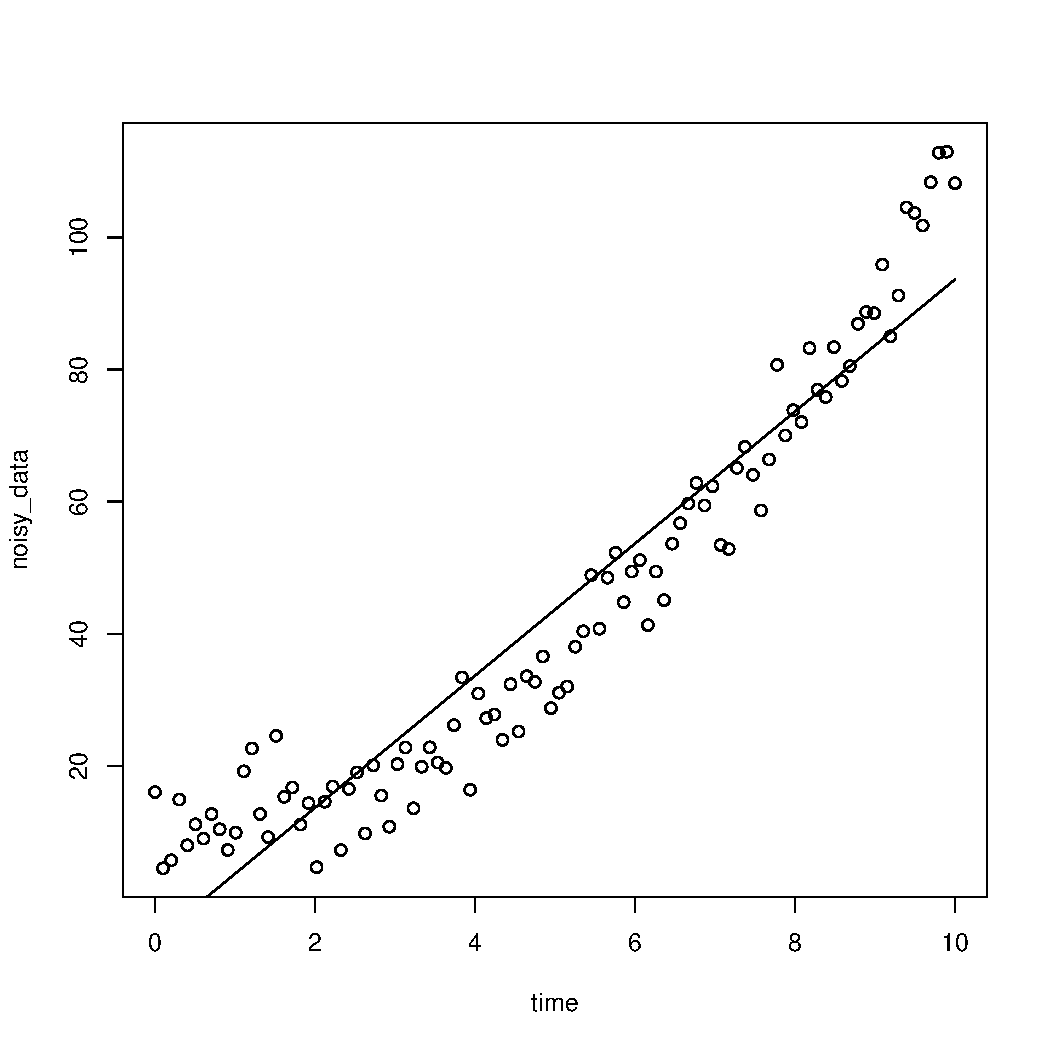
\includegraphics[scale=0.5]{linear_model}
\caption{Our first shot at fitting some data.}
\end{figure}

To see this in more depth, we may call \verb|plot(linearmodel)| which produces several plots of the data. This further indicates the model is biased at the endpoints, suggesting a linear model isn't ideal. Of course, 

To fit a nonlinear curve to the data we must use a different function, \verb|nls| (nonlinear least squares). Here is how that would be performed:
\begin{Verbatim}[frame=single, fontsize=\small]
quadratic <- noisy_data ~ p1*time^2 + p2
model <- nls(quadratic, start = list(p1=0, p2=0))
# Plot the new, least-squares quadratic
p1 <- coef(model)[1]
p2 <- coef(model)[2]
curve(p1*x^2 + p2, from = lb, to = ub, add = TRUE)
\end{Verbatim}
% To add:

% Plot & save plot output as NOT A PDF!
% Save output to a file
% The Resources section contains a link to a web page describing the \verb|par| function, which can be thought of as \emph{parameters} for plotting. Because of R's default function arguments, you will almost never have to worry about all of the dozens of parameters.

In this case we can look at the plots and see that a quadratic model fits better.

% TODO: This above too detail oriented and is not really relevant

\subsection{Plotting}\label{plotting}
R has very powerful plotting features. They are described as ``beautiful'' by data visualization geeks. One reason for this is that R can output in vector formats, which is to say they scale to any size. R supports many filetypes, but this guide uses the pdf format by calling the \verb|pdf| function. Two more useful filetypes supported are png and jpg, which are called identically to the pdf driver, only using the \verb|jpeg| and \verb|png| functions.

This section will explain the various uses of the \verb|plot| and \verb|curve| functions used in the previous subsection and expand upon them to produce more sophisticated graphs.

Now, suppose we have already created all the required data and gone to assemble a plot like so: (this is simply a compilation of previously shown commands)
\begin{Verbatim}[frame=single, fontsize=\small]
plot(time, noisy_data)
curve(slope * x + intercept, add = TRUE)
curve(p1*x^2 + p2, add = TRUE)
\end{Verbatim}

The optional parameter \verb|add = TRUE| states that the curve should be added to an existing plot. The default is false, which is to say each call to \verb|curve| creates a new plot. Now, let's make these plots a bit nicer.

\begin{Verbatim}[frame=single, fontsize=\small, numbers=left]
pdf("sample_plot.pdf") 

# Make the scatterplot and label the axes
plot(time, noisy_data, xlab = "Time (months)",
     ylab = "Number of Cats (millions)")
# Change the title and marginal text
title("Number of Cats Over Time", line = 2, cex.main = 1.6)
mtext("What do we do with all these cats?\nBy Sam Pollard", font = 3,
      cex = 0.8)
# Overlay the linear and quadratic best fit curves
curve(slope * x + intercept, add = TRUE, lwd = 2, col = "red")
curve(p1*x^2 + p2, add = TRUE, lwd = 2, col = "blue")
# Create the legend
quadtext <- paste0(format(round(p1, 2), nsmall = 2), " t^2 + ",
                   format(round(p2, 2), nsmall = 2))
linetext <- paste0(format(round(slope, 2), nsmall = 2), " t + ",
                   format(round(intercept, 2), nsmall = 2))
legendtext <- c(quadtext, linetext)
legend("topleft", legend = legendtext, col = c("blue","red"), lwd = c(2,2))
# Say that we're finished plotting so the pdf can be saved
dev.off()
\end{Verbatim}

This is a lot of code to take in at once but it will be broken down. The first call to plot on line 4 plots time against the data. The x and y labels are changed from their default (the variable names) to something sillier. For line 6, the \verb|line| parameter sets where the title should appear, as determined from an offset from the top of the graph. That is, \verb|line = 2| is two ``units'' above the top of the graph, while \verb|line = -2| would be two units down from the top, so inside of the graph. Exactly what determines a unit is up to R to decide. In general, it is a good idea to trust R in what looks nice. One must give up a little freedom for convenience, knowing that things are done in R for good reason. The second parameter \verb|cex.main| stands for ``character expansion of the main text.'' This means that, relative to the default size 1, the title is 1.6 times larger than that.

Line 8 creates ``marginal text'' and the parameters are a bit cryptic. The \verb|\n| in the middle of my string is a newline, so my name appears under the ``Cats'' query. Setting \verb|font = 3| means italic, and \verb|cex = 0.8| shrinks the text a bit. 

Lines 11 and 12 overlay curves on the scatterplot. The first argument is a general form for a function: notice that \verb|x| is not a variable which has a value associated with it. This allows functions to be plot. The \verb|lwd| parameter stands for ``line width'' and is again a multiple of the default value 1.

Next, the legend is created. This is done in several steps so the R command doesn't get too messy. The \verb|quadtext| and \verb|linetext| store the string which represents the equation. There are many ways to do this, and R does support mathematical equations. However, I used the \verb|paste0| function. Recall that \verb|paste| allows concatenation of strings. However, in the previous usage, we created a vector. Next, \verb|paste0| is simply a convenience and is identical to \verb|paste(..., sep="", collapse=TRUE)|. That is, this function combines everything you give it into a single string. The \verb|round| function is as one would expect: rounding a value to 2 decimal places. The second argument to \verb|format| gives the minimum number of digits to the right of the decimal place.

To create the legend, one must first specify the location. I chose the top left corner, but there are also options such as \verb|top|, \verb|bottomright|, or by the x and y coordinates. Notice that all the parameters afterwards are vectors created using the ubiquitous \verb|c| function. Thus, the first element of each parameter will correspond to the first line and text to be displayed with that line.

Lastly, once you're satisfied with the graph the function \verb|dev.off()| turns off the device which is displaying the plot which causes the file to be written to the location specified by \verb|pdf|. Running this script will cause a file called \verb|sample_plot.pdf| to be saved in the \emph{working directory} that R is running in. To specify exactly where the plot should be saved it is best to use an absolute file location. For example:
\begin{verbatim}
pdf("C:\Users\Sam Pollard\Documents\R\sample_plot.pdf")
\end{verbatim}
All this combined makes the graphic shown in Fig. 1 

\begin{figure}[ht]
\label{quadratic}
\centering
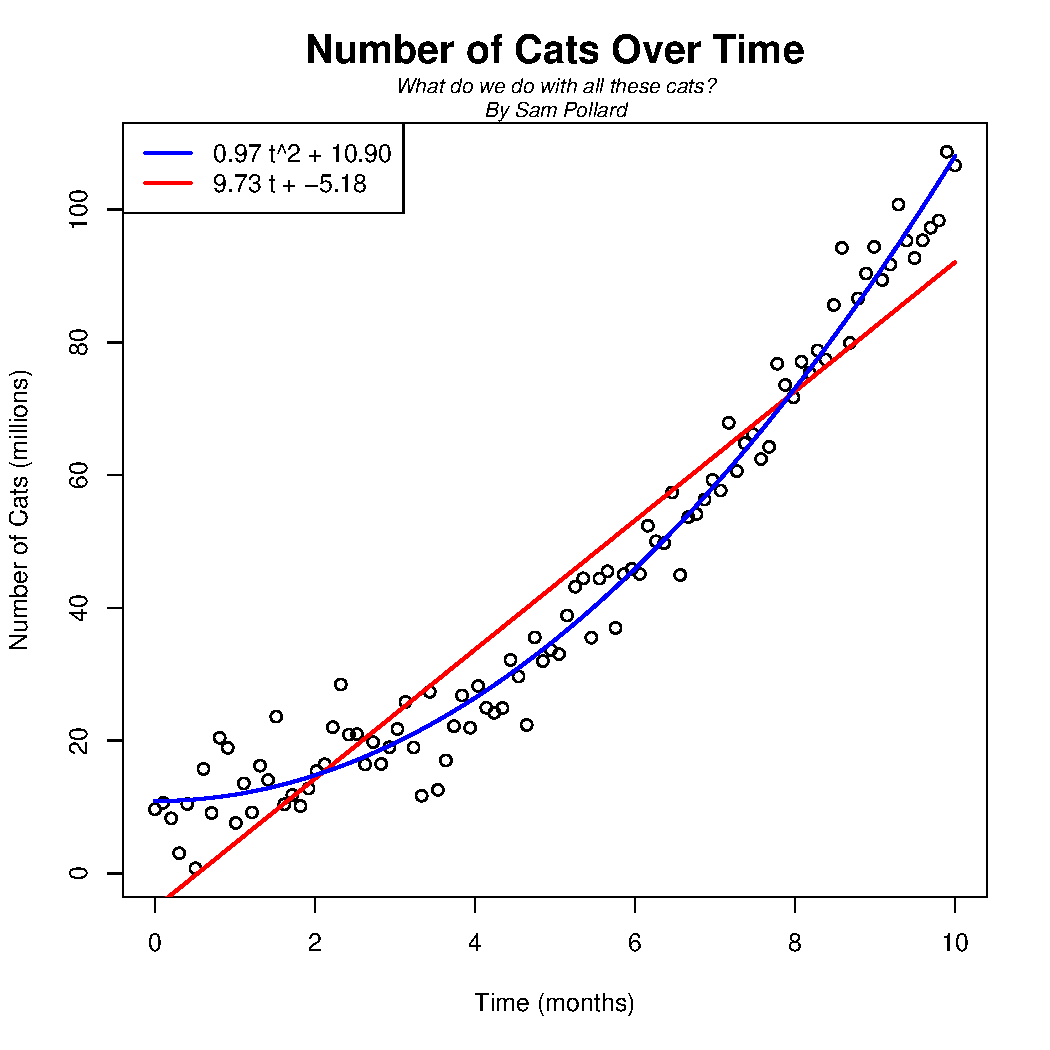
\includegraphics[scale=0.6]{sample_plot}
\caption{The figure created in Section \ref{plotting}.}
\end{figure}

% One final function which I will describe is the \verb|par| function. This both allows setting and saving of graphing parameters. These are passed into par like any other function argument, and typing \verb|oldpar <- par()| stores the current parameters for saving later and to restore them one would type \verb|par(oldpar)|. Typing \verb|?par| is both an enlightening and intimidating experience. There is page after page of options. Fortunately, many of these options generalize to other plotting functions. For exampke, you'll notice that I used \verb|col| in the \verb|legend| function. This is can be used to specify colors of many different parameters in \verb|plot|.

% Other functions: axes
% Maybe add later: date in the corner, explain all the crazy code I just did.

\section{Conclusion of Part I}
This concludes the first part of the guide. You are missing many important aspects of programming in general. Much of what makes a programming language a programming language is missing: the \verb|if| and \verb|for| statements, creating custom functions using \verb|function|, and much more. This is firstly a practical guide and even without those fundamental features a lot can be done with R.

\clearpage
\part{Learn You Some R, ``In Theory''}
\textbf{Note: This part of the guide is far from complete.}

This part of the guide attempts to give some general programming knowledge as opposed to some useful tricks. This can be thought of as learning how to build a fishing rod instead of learning how to fish. The benefit to the theoretical side is these concepts apply to every other programming language. The drawback is even if you know how to build a fishing rod, you can still be a terrible fisher.

\section{Functions}\label{functions}
It is difficult to give a meaningful definition of a function, but the best I can come up with is, ``a function is an object which takes as input zero or more arguments, performs some operations based on these arguments, and then returns a value or nothing.'' So, what is a function?

Incredibly useful, as it turns out. Without getting into too much detail, it has been proven that \emph{everything} computers can be made to do can be boiled down to computing functions and setting variables\footnote{If you would like to learn more, this is referred to as Lambda Calculus.}. This is motivation to understand both variables and functions.

Now, let's start by creating our own function in R. Suppose we just want to take any vector as input, and enclose that in parentheses.

\begin{Verbatim}[frame=single, fontsize=\small]
parenthesize <- function(x) {
	interior <- paste(x, collapse = " ")
	return(paste("(", interior, ")"))	
}
\end{Verbatim}
Notice that this looks like variable assignment. In fact, this is exactly what is happening. Next up we see the braces \verb|{}|. All these do is define what is inside the function. We most likely have functions which take up multiple lines of source code, so the braces show exactly when the function begins and ends. It is proper style to indent everything between sets of braces. This makes the code more readable because there may often be multiple levels of braces which can get incredibly confusing even with proper indentation.

Now the function \verb|parenthesize| is \emph{bound} to the variable \verb|parenthesize| and we can use it like we would use any other built in function:
\begin{verbatim}
> parenthesize(c(1,2,3,4))
[1] "( 1 2 3 4 )"
\end{verbatim}

The variable \verb|interior| in this context has what's called a \emph{scope}. This is an important concept in programming and refers to when you can access particular variables. For example, once we define the function, if we try to access \verb|interior| outside of the braces defining the function we get an error:
\begin{verbatim}
> interior
Error: object 'interior' not found
\end{verbatim}
This is because \verb|interior| is local to the function \verb|parenthesize|. This helps keep the set of all active variables less cluttered, and makes things easier because you can reuse variable names such as \verb|x|. On the topic of \verb|x|, by making it an argument to \verb|parenthesize|, we are making the variable \verb|x| only in scope between the braces following the key word \verb|function|. That is, whatever the value of \verb|x| gets inside of the function is forgotten when the function returns. This is useful because we can now pass anything into \verb|parenthesize| and it will always be known as \verb|x| inside of the function. Even if we had a variable called \verb|x| that we were using \emph{outside} of the function definition, this would be temporarily \emph{shadowed}, or eclipsed by the \verb|x| specified as \verb|parenthesize|'s input argument.

% TODO: Have example of this later? Add a section called scope?
% This means we don't have to worry about anything else which may happen to be named \verb|x|. Once we leave the safety of the \verb|}|, we can again refer to the old \verb|x| which

A large part of programming is formatting data correctly. We have seen that \verb|read.csv| attempts to make this easier with its \verb|sep| argument. This allows us to deal with an arbitrary separator for a csv file. However, many other applications are not as forgiving. For example, a URL must be in a very specific format to get to the correct page. As a motivating example, suppose we have the following protein IDs (as recognized by the RCSB Protein Data Bank) and wish to convert these into a comma-separated list:

\begin{Verbatim}[frame=single, fontsize=\small]
> # The input
> proteins <- c("3G73","3CO6","1VDE","1AF5","1EVX","2OST","1QQC","1KN9","3BF0")
> # The desired output
> protein_string <- "3G73,3CO6,1VDE,1AF5,1EVX,2OST,1QQC,1KN9,3BF0"
\end{Verbatim}

The reader may notice that the variable \verb|proteins| is basically already a comma-separated list. Suspend your disbelief and suppose that we don't already know \verb|proteins|, or that you don't want to remove all of those quotes around each protein ID. Our goal then is to have some function \verb|intersperse| which takes as input a vector and outputs that vector with commas in between the entries. So instead of typing the value of \verb|protein_string| out by hand like I did when writing this guide, we could get the same result with a function.

% TODO: Write it the bad way

\begin{Verbatim}[frame=single, fontsize=\small]
intersperse <- function(vec, ele) {
	y <- vector("character", length = 2*length(vec) - 1)
	# What if the length of vec is less than 2?
	y[seq(2, length(y), 2)] <- ele
	y[seq(1, length(y), 2)] <- vec
	return(paste0(y, collapse = ""))
}
\end{Verbatim}

Full disclosure: There is a much simpler way to do this. We have seen the \verb|paste| function before, and the \verb|collapse| argument. Now, what if we just let R handle the hard work for us?

\begin{Verbatim}[frame=single, fontsize=\small]
intersperse <- function(vec, ele) {
	return(paste(vec, collapse = ele))
}
\end{Verbatim}

Now, using \verb|intersperse| we get
\begin{verbatim}
> protein_string_with_intersperse == intersperse(proteins, ",")
> protein_string_with_intersperse == protein_string
[1] TRUE
\end{verbatim}
What I just showed you was the first test case.

\newpage
\part{Exercises}

Just as you cannot learn how to play piano by watching someone else play, you cannot learn to program by watching (or reading about) someone else program.

\begin{enumerate}
	\item { Write your own \verb|head| function. Call this function \verb|Head|. Notice that this is considered an entirely different function in R. This is because R is case sensitive. Likewise, the variable \verb|X| is different from \verb|x|. Recall that \verb|head| takes as input some object and outputs the first few rows (or elements) of that object. Test your function on the following inputs:
	\begin{verbatim}
		Head(seq(1000))
		data(Puromycin) # Load in a sample data.frame
		Head(Puromycin)
		Head(5)
	\end{verbatim}
	Make sure this matches the ouput of calling \verb|head| with the same inputs.
	}

\end{enumerate}

% A less stupid function would be to intersperse

% Exercise: Create a function which takes in a full name and returns the name with the last name followed by first initial.
% For example,
% Sam Pollard would be returned as Pollard S.
% How would you test that this is correct? What about strange names like Johannes van der Waals?
\clearpage
\section{Resources}
Arguably the most useful resource you can make use of in R is the \verb|help| function. You pass \verb|help| any function as an argument, which will direct you to an online help source. For example, \verb|help(rbind)|. This is the same as \verb|?rbind|.

Here are some other resources. I have not cited every one of the sources I used when creating this guide, but the ones omitted were almost all from stack exchange, the R documentation, or Wikipedia. Thus this can be also thought of as a partial bibliography.
\begingroup
\renewcommand{\section}[2]{}%
%\renewcommand{\chapter}[2]{}% for other classes
\begin{thebibliography}{}
	\bibitem{Learnxinyminutes}
		\url{http://learnxinyminutes.com/docs/r/}
		This is a pretty basic guide but is the easiest to follow.
		
	\bibitem{mycode}
		\url{https://github.com/sampollard/pcrystal}
		This is some of my own R source code.
		
	\bibitem{shortref}
		\url{http://cran.r-project.org/doc/contrib/Short-refcard.pdf}
		This is a useful cheat sheet. Much of it won't make sense right away, but will help you with commonly-used functions.
		
	\bibitem{rintro}
		\url{http://cran.r-project.org/doc/manuals/R-intro.pdf}
		This is a more in-depth guide to R. Notably, chapter 12 contains a lot of good information on graphics.
	
	\bibitem{nlsexample}
		\url{http://www.walkingrandomly.com/?p=5254}
		I used this reference in my nonlinear regression example.
		
	\bibitem{advgraph}
		\url{http://www.statmethods.net/advgraphs/} Provides explanation of many of the parameters of the \verb|par| and \verb|plot| functions.
\end{thebibliography}
\endgroup

\end{document}
